\section{Goals and Methodology}
The IDDR implementation uses the \texttt{Linux kernel 3.5.0} for both application and driver domains. We tested it with Arch Linux on \texttt{x86\_64} platform. The specification of the system used for evaluation is presented in the table~\ref{tab:config}. 

\begin{center}
\begin{tabular}{|r|l|} 
  \hline
  \label{tab:config}
  System Parameter & Configuration \\
  \hline
  Processor & 2 X ??, ??.?? Ghz \\
  Number of cores & 4 per processor \\
  Hyperthreading & ?? \\
  Turbo boost & ?? \\
  L1 L2 cache & ??K/??K per core \\
  L3 cache & ?? X ??MB \\
  Main memory & ??GB \\
  Storage & SATA, HDD ??RPM \\
  \hline 
\end{tabular}
\end{center}
 
\subsection{Goals}
\label{sec:goals}
Our evaluation contains 
\begin{enumerate} 
\item comparison of Xen split driver and IDDR without any performance improvement, 
\item an evaluation of IDDR performance improvement over base IDDR system,
\end{enumerate}
The goal of this evaluation is to show that by avoiding the use of event channel in communication channel improves the performance of the system. 
\\[3mm]
SATA disk has the most general use case and loop device being a fileIO operation, ramdisk being a fastest block device; these all three block devices cover the range we would want to run performance test for both Xen driver domain system and IDDR system. 
\\[3mm]
In order to do performance measurement, we format the raw block device with the ext2 file system, and run the fileIO SysBench benchmark~\cite{sysbench} on it. Sysbench benchmark generates 128 files with \texttt{1Gb} of total data and performs random reads, random writes and mix of random read-writes with a block size of \texttt{16Kb}. 

\section{Xen split driver vs IDDR}
In this thesis we re-implement the xen driver domain, and improve the performance of the xen driver domain by introducing spinlocks instead of event channel interrupts in communication channel. In order to show the performance improvement in the system, we compare the improved results with the base IDDR system. However, without comparing the base IDDR with Xen driver domain, it won't be fair to claim that the new improved IDDR system performs better than Xen driver domain. In this section, we show that the performance of the base IDDR system and the Xen driver domain is same. Hence, any performance improvement over the base IDDR system can be claimed as the performance improvement over the xen driver domain.
\\[3mm]
As explained in the chapter 2, xen driver domain follows the architecture of Xen split driver. In order to measure the performance of the Xen driver domain, we run performance benchmarks on a block device which uses with Xen split driver.

\subsection{Experimental setup}

\subsubsection*{Xen split driver}
We create a ramdisk in domain 0. The guest domain domU is configured to use the ramdisk as a disk through split block device driver. We do similar setup for the loop device and the SATA disk. For example, in case of loop device, we create a loop device in domain 0 and then configure the guest domain to use loop device as a disk. In case of SATA disk, we configure the guest domain to use SATA disk as a secondary disk. We format and mount the the raw disk in guest domain with the ext2 file system. Sysbench benchmark is run on the mounted partition as explained in section~\ref{sec:goals}.

\subsubsection*{IDDR}
In xen split block device driver setup, the back end device driver runs in a domain 0 and the front end device driver runs in the domain U. HVM guests are expected to have less syscall overhead and faster memory bandwith than PV guests. Our setup is configured such that the domain U is a HVM guest and the domain 0 is a PV guest. In order to have fair comparision it is necessary to run the back end driver in the domain 0 and the front end driver in the domain U.
\\[3mm]
We insert a ramdisk and front end module in the domain 0. The back end module is inserted in the guest domain domU. We format and mount the ramdisk with ext2 file system and sysbench benchmark is run on it.  
\\[3mm]
Similar setup is used for loop device and SATA disk.
\subsubsection*{Comparision}
\begin{figure}[!ht]
\centering
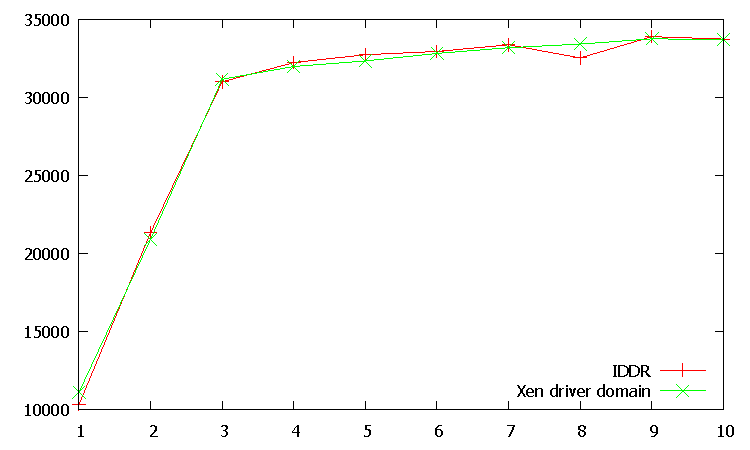
\includegraphics[scale=1]{iddrvsxen-ramdisk-rdwr}
\caption{IDDR vs Xen split driver}
\label{fig:iddrvsxen-ramdisk-rdwr}
\end{figure}
\begin{figure}[!ht]
\centering
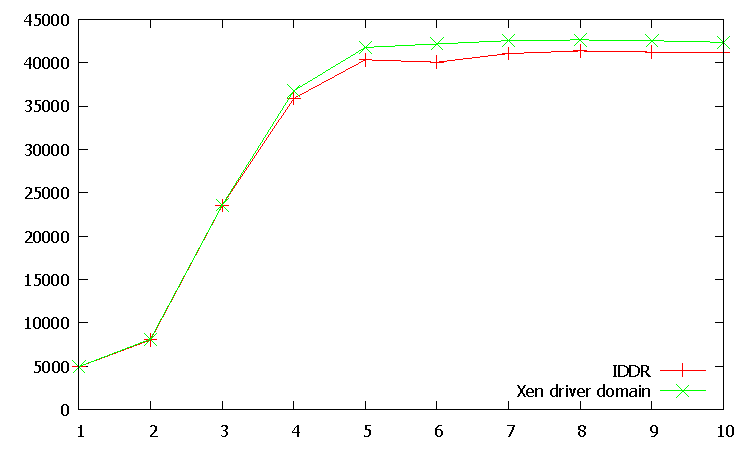
\includegraphics[scale=1]{iddrvsxen-loop-rd}
\caption{IDDR vs Xen split driver}
\label{fig:iddrvsxen-loop-rd}
\end{figure}
Figure~\ref{fig:iddrvsxen-ramdisk-rdwr} shows the performance of random reads-writes on a ramdisk, and figure~\ref{fig:iddrvsxen-loop-rd} shows the performance of random reads on a loop device. Both systems provide roughly similar performance. The figures show that the performance of the IDDR is similar to Xen driver domain. In further section we evaluate the performance improvement against IDDR system.

\section{IDDR performance improvement}
We measure and compare the performance of the base IDDR system (event channel interrupt) and the new imrpoved IDDR system (Spinlock). We run the fileIO sysbench benchmark with random reads, random writes and mixed random reads-writes. 
\subsection{Experimental setup}
In the setup, domain 0 is a Application domain, and domain U is a driver domain. A ramdisk is created in the domain U (driver domain). The back end module is inserted in the domain U (driver domain) and the front end driver is inserted in the domain 0 (application domain). The raw disk is formatted and mounted with ext2 file system in application domain. Sysbench benchmark is run on the mounted partition. 
\\[3mm]
For loop device similar setup is created. We create a loop device in a driver domain, and insert back end driver in the driver domain. Front end driver is inserted in domain 0. For SATA disk, we passthrough SATA disk to driver domain, so that driver domain can directly access the SATA disk. 
\subsubsection*{Comparision}
\begin{figure}[!ht]
\centering
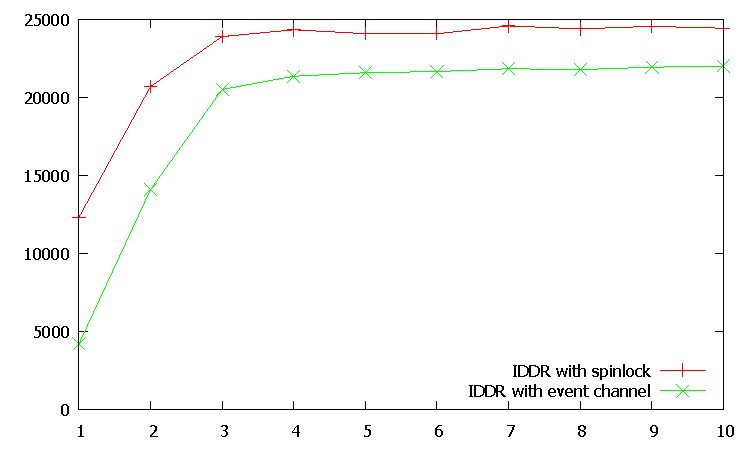
\includegraphics[scale=1]{threadvsspin}
\caption{IDDR with Spinlock vs IDDR with event channel}
\label{fig:threadvsspin}
\end{figure}
Figure~\ref{fig:threadvsspin} compares the performance of the base IDDR and the new improved IDDR with random reads-writes on a ramdisk. The figure shows that the new IDDR system implementation with spinlock performs better than the base IDDR implementation. 
\pagebreak

% ref
\ifbool{toShowBibliography}{\bibliography{references}}{}